\chapter{Implementation Details}
\label{chap:Implementation Details}
\ffigure{img/implementation.png}{A simple spatial join algorithm that puts elements into buckets based on their position in a grid. By putting data pointers directly in the buckets instead of referring to a linked list, a layer of indirection is removed, and 3-fold improvement is observed. Courtesy of \cite{Sidlauskas2014-ef}.}{fig:implementation}

As we move up the memory hierarchy, careful implementation becomes more important. Recent work by Sidlauskas \ea~claims that for in-memory databases, there is a challenge in concluding about data structures and algorithms only; the implementation also plays a significant role in performance \cite{Sidlauskas2014-ef}. For instance, if an extra layer of indirection is removed for an algorithm, as seen in Figure \ref{fig:implementation}, we observe a 3-fold performance improvement. 

We have decided to dedicate an entire chapter to \textit{implementation details}, and explain how performance can be improved by reducing the number of branches, avoiding layers of indirection, and utilizing CPU caches. We will first cover basic CPU theory, and then study related techniques employed by systems studied in this research.

\newpage

\section{Background Information on Modern CPUs and Compilers}
\label{sec:Background Information on Modern CPUs and Compilers}
Modern processors are capable of performing an enormous amount of calculations per second, but that depends on the amount of available and independent work. The instructions-per-second (IPC) difference between minimal and maximal CPU utilization can easily be an order of magnitude \cite{Boncz2005-wj}. Hence, database software must be implemented such that it fully exploits the processing power made available by the CPU.

\subsection{Pipelining, Superscalar Processing, and Independent Instructions}
\label{sub:Pipelining, Superscalar Processing, and Independent Instructions}
\afigure{img/superscalar.png}{A simple superscalar pipeline. Multiple execution units allows for processing multiple instructions in parallel. Courtesy of \cite{Wikipedia_contributors2015-kp}.}{fig:superscalar}{0.6} 

Modern processors improve clock rate and IPC by using a technique known as \textit{pipelining} \cite{Boncz2005-wj}. By dividing an instruction execution into multiple steps, there is less work per stage, and the CPU frequency can be increased. Figure \ref{fig:superscalar} depicts an example pipeline with five stages. However, pipelining also introduce two dangers; \textit{instruction dependencies} and \textit{branch misprediction}.

In a pipeline, \textit{dependencies between instructions} impose a problem. If an instruction is dependent on another, it must wait for the other instruction to complete before it enters the pipeline. Dependent instructions can severely hurt performance, especially if the pipeline is long.

Conditional branches are also affected by dependencies between instructions. When executing a conditional branch instruction, the decision whether to take a branch is usually dependent on the result of a preceding instruction \cite{Boncz2005-wj}. To avoid stalling the pipeline when waiting for the expression to evaluate, modern CPUs use a technique known as branch prediction where the processor immaturely starts executing the branch that is most likely to be taken. The performance penalty occurs if a branch is \textit{mispredicted}, where the instructions in the pipeline must be invalidated (pipeline flushing).

Another way that performance is increased in a processor is by having muliple execution units. We refer to such processors as \textit{superscalar}. As seen in Figure \ref{fig:superscalar}, a superscalar processor can have multiple instructions in the same stage of the pipeline, which allows for for IPC (instructions per cycle) $> 1$. However, for this functionality to be fully utilized, independent work is required.

\begin{figure}
  \centering
  \begin{subfigure}{0.45\textwidth}
    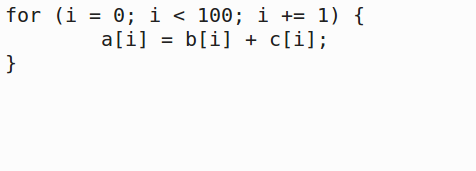
\includegraphics[width=\textwidth]{img/loop-unrolling-1.png}
    \caption{Original loop}
    \label{fig:loop-unrolling-1} 
  \end{subfigure}
  \begin{subfigure}{0.45\textwidth}
    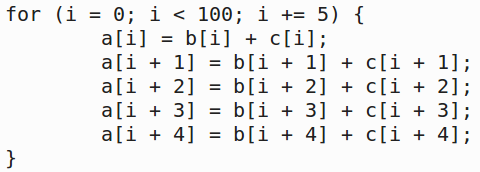
\includegraphics[width=\textwidth]{img/loop-unrolling-2.png}
    \caption{Unrolled loop}
    \label{fig:loop-unrolling-2} 
  \end{subfigure}
  \caption{By unrolling loops, instructions are made independent and the number of branches is reduced.}
  \label{fig:loop-unrolling} 
\end{figure}
Hence, to reach maximum performance on a pipelined, superscalar processor, we must find independent work. Since most programming languages do not let the programmer specify which instructions are independent of each other, compiler optimizations play a critical role in CPU utilization \cite{Boncz2005-wj}. The most widely used technique used by the compilers to address this challenge is through \textit{loop unrolling}, which is used to reduce the number of branches and increase independence between instructions \cite{Wikipedia_contributors2015-zc}. As seen in Figure \ref{fig:loop-unrolling}, loop unrolling reduces the number of iterations in a loop (reduction of branches) and replaces it with multiple instances of the same instruction. If the instructions are independent, they can be processed in parallel.

\subsection{CPU Caches}
\label{sub:CPU Caches}
Since transfering data from main memory to CPU can take around $~200$ cycles, modern CPUs utilize multiple layers of on- and off-chip caches to reduce this latency. Efficient usage of caches is paramount for CPU throughput, since roughly 30\% of all instructions in a program are memory loads or stores \cite{Boncz2005-wj}. We know that IPC for DBMSes is strongly impaired by cache misses, and cache utilization is an important topic for in-memory databases \cite{Exasol2014-xh}.

The best way to tackle this challenge is to design algorithms and data structures that are \textit{cache aware} \cite{Farber2012-vh}. Designing such programs is out of the scope of this report, but it briefly boils down to two things:
\begin{itemize}
  \item \textit{Coordinate temporal and spatial locality}. Data processed together should be stored at consecutive memory addresses. Code locality is also important \cite{Neumann2011-uq}.
  \item \textit{Avoid false sharing of cache lines}. Multiple cores in a processor should not write to data belonging to the same cache entry at the same time to avoid unecessary invalidations.
\end{itemize}
\textit{Compression}, which we described in Chapter \ref{chap:Data Compression}, and \textit{vectorized execution}, which we discuss in Section \ref{sec:Loop Pipelining and Vectorized Execution}, are two techniques used to improve cache performance \cite{Larson2013-mc, Lemke2010-is}.

\textit{Prefetching} is another method used to increase cache utilization. Prefetching proactively loads data into caches such that the data is available when an instruction needs it.

\subsection{Call Stack and Subroutine Invocations}
\label{sub:Call Stack and Subroutine Invocations}
\afigure{img/call-stack.png}{A call stack for a program in execution. Each stack frame contains input parameters, function return address, and local variables for a subroutine invocation. Courtesy of \cite{Wikipedia_contributors2015-od}.}{fig:call-stack}{0.5}

A \textit{call stack} is commonly used in a computer program to store information and state about active subroutines \cite{Wikipedia_contributors2015-od}. Each time a subroutine is called, a \textit{stack frame} is added to the call stack that stores the input arguments, return address, and variables local to the subroutine. See Figure \ref{fig:call-stack}. The call stack can be implemented in both hardware and software, and the implementation varies between different systems. This stack-based technique implies that calling a subroutine comes at a cost; registers must be stored on the stack, and a new stack frame must be added.

Trading off time with space is usually done to address the above challenge; adding more code to improve program efficiency. \textit{Function inlining} is a technique used by compilers where the subroutine code is copied into the callee's body. This way, no new stack frame is created for the subroutine, avoiding the overhead associated with a function invocation.

\textit{Macro expansion} is another form of code generation. Macros are normally specified by the application programmer, and can be used for programmer-controlled inlining of functions or constant values. Macros can also be used to generate multiple versions of function or class definitions (templating), a technique commonly used to let a single implementation support different data types.

\section{Branch Avoidance}
\label{sec:Branch Avoidance}
\ffigure{img/branch-selectivity.png}{Predicate evaluation performance for queries with different query selectivities. A \textit{branch version} and a \textit{predicated version} is tested. For the AthlonMP processor, the branch version are 2-3 times slower on queries with 40\%-60\% selectivity, while the Itanium2 processor has constant processing time. The predicated version offers constant processing time for both processors. Courtesy of \cite{Boncz2005-wj}.}{fig:branch-selectivity}

We saw in the previous section that branches should be avoided due to the penalties of branch misprediction. Besides, branches also cause dependencies between instructions. 

The consequences of inaccurate branch prediction are studied by Neumann \ea~\cite{Neumann2011-uq}. In this research, the performance of queries with various selectivities was tested. As we can see in Figure \ref{fig:branch-selectivity}, queries with 40\%-60\% selectivity executed on an AthlonMP processor are roughly 2-3 times slower than queries with selectivities close to 0\% or 100\%. Hence, selectivity can severely affect the query performance. The Itanium2 processor does not have the same characteristic, as the Itanium architecture allows for both \textit{not taken} and \textit{taken} branches to be executed simultaneously.

Neumann \ea~also developed a branchless version (predicated version) to evaluate predicates in the queries. The branchless variant is denoted as \texttt{predicated version} in Figure \ref{fig:branch-selectivity}. For both AthlonMP and Itanium2 processors, this implementation offers constant performance for all selectivities, but is, in general, more expensive.

Branch avoidance is also important in other parts of the system, for instance when decompressing. Zukowski \ea~present a decompression algorithm that is free for \textit{if-then-else} statements \cite{Zukowski2006-oz}. By running the algorithm in two tight loops instead of one, branch misprediction is reduced, and the loops can be pipelined by a compiler.

Branches can also be avoided by compiling queries to machine code \cite{Lamb2012-kg}. We will elaborate on this technique in Section \ref{sub:Compiling Queries to Machine Code}.

\subsection{Short-circuiting}
\label{sub:Short-circuiting}
\begin{figure}
  \centering
  \begin{subfigure}{0.45\textwidth}
    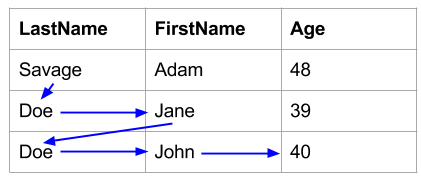
\includegraphics[width=\textwidth]{img/short-circuiting-1.png}
    \caption{Short-circuiting}
    \label{fig:short-circuiting-1} 
  \end{subfigure}
  \begin{subfigure}{0.45\textwidth}
    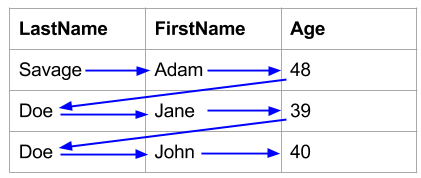
\includegraphics[width=\textwidth]{img/short-circuiting-2.png}
    \caption{No short-circuiting}
    \label{fig:short-circuiting-2} 
  \end{subfigure}
  \caption{Predicate evaluation for query \texttt{WHERE LastName='Doe' AND FirstName='John' AND Age>21}. (a) skips evaluating rest of the predicates if one predicate is false, while (b) evaluates all predicates regardless of previous results.}
  \label{fig:short-circuiting} 
\end{figure}
\textit{Short circuiting} is referred to a special case of Boolean operator evaluation in which the next argument is not evaluated if the current argument is sufficient to determine the value of the expression \cite{Wikipedia_contributors2015-rk}. Figure \ref{fig:short-circuiting} illustrates the difference between short-circuit and non-short-circuit predicate evaluation. In short-circuiting, the scan proceeds to the next tuple as soon as one predicate is false, as opposed to the verision without short-circuiting that evaluates all predicates regardless of previous results.

Since short-circuit boolean operators are control structures and not simple arithmetic operators, there is a chance of branch misprediction. That is why \blink~\cite{Raman2008-gi, Johnson2008-cp} does not short circuit between tuples. If a block is selected for scanning, all fields in a record are checked. According to Raman \ea, short-circuiting only improves performance on low selectivity queries \cite{Raman2008-gi}.


\section{Loop Pipelining and Vectorized Execution}
\label{sec:Loop Pipelining and Vectorized Execution}
The absence of loop pipelining can have dramatic effects on query performance \cite{Boncz2005-wj}. Boncz \ea~show that \mysql~uses 49 cycles per tuple because loops are not unrolled. In this system, tuples are processed one at a time with 1-2 function calls to extract the needed data from a tuple per iteration \cite{Abadi2008-dd}. Besides, evaluating a predicate is usually a small operation compared to the overhead associated with calling subroutines. In other words, most of the 49 instructions are spent managing the call stack or waiting for instruction dependencies.

To ensure proper loop pipeline behavior, compilers must be aware that pointers do not overlap, such that loop unrolling can be used \cite{Boncz2005-wj}. Operations in \monetx~are compiled with compiler hints that tell the compiler that processing a tuple is independent of the others. In standard \textit{C} compilers, this can be done by using the \texttt{\_\_restrict\_\_} pointer type.


\subsection{Vectorized Execution}
\label{sub:Vectorized Execution}
To avoid unnecessary subroutine invocation overhead and help the compiler identify which instructions are independent, \textit{vectorized execution} is normally used. Vectorized execution, or block iteration, is the technique where multiple rows are processed at the same time to avoid the overhead associated with tuple-at-a-time processing \cite{Abadi2008-dd}. Vectorized execution enables loop unrolling, memory prefetching, and minimizing of cache misses \cite{Larson2013-mc}. Research performed by Abadi \ea~shows that vectorized execution in columns stores improves performance by 50\% on average.

% explain who uses it
Several systems studied our research use vectorized execution. \ibm~and \mssql~work on batches of thousands of row at a time \cite{Larson2013-mc, Raman2013-em}. \monetdb~and \monetx~use vectors instead of single values as their primary structure for storing data \cite{Boncz2005-wj, Boncz2002-yj}. Vectorized execution is also used by \cstore~and \blink~\cite{Johnson2008-cp, Stonebraker2005-qz}.

% Explain how it works.
\afigure{img/vectorized-execution.png}{\mssql~operators work on row batches. Each row batch contains thousands of rows stored as column vectors. Also, a bit vector indicates which rows that qualifies for a query. Courtesy of \cite{Larson2013-mc}.}{fig:vectorized-execution}{0.4}
In vectorized execution, blocks of values from the same column are sent to an operator for evaluation \cite{Zukowski2006-oz}. Query operators in \mssql~work on row batches, batches that contain thousands of rows stored in a column format. In addition to the column vectors, an additional \textit{qualifying rows vector} is used to indicate which rows that have been logically purged from the batch when executing a query. Figure \ref{fig:vectorized-execution} shows this structure.

Regarding the size of the vectors in vectorized execution, we have found that vectors should not be too small due to increased overhead and less parallelism, nor too big, as it should fit in CPU cache \cite{Boncz2005-wj}.

Although vectorized execution for column stores normally outperforms tuple-at-a-time query processing, there are some disadvantages by using this model. Neumann \ea~claim that vectorized execution eliminates a major strength of the iterator model, namely \textit{pipelining} \cite{Neumann2011-uq}. In this context, pipelining means the ability for an operator to pass tuples to its parent operator without copying the value. When vectorized execution is used, intermediate results have to be stored somewhere (materialized), which consumes memory bandwidth. Neumann \ea~address this issue by compiling queries into machine code, a technique we study in Section \ref{sub:Compiling Queries to Machine Code}.

\section{Code Generation}
\label{sec:Code Generation}
In Section \ref{sub:Call Stack and Subroutine Invocations}, we briefly discussed how code generation can be used to avoid overhead related to function invocations. Besides, code generation can also reduce branches and improve cache performance. In this section, we study two code generation techniques employed by systems studied in this research.


\subsection{Compiling Queries to Machine Code}
\label{sub:Compiling Queries to Machine Code}
Compiling queries to native machine code can be used to increase the performance of expression evaluation, avoid branches, and reduce the number of function calls \cite{Lamb2012-kg, Neumann2011-uq}. It is particularly effective for ad-hoc queries \cite{Psaroudakis2014-ma}, which we know that \bd~queries are. Systems compiling queries into machine code include \blink~\cite{Barber2012-xt}, \ibm~\cite{Raman2013-em}, \vertica~\cite{Lamb2012-kg}, \hyper~\cite{Psaroudakis2014-ma}, and \mssql~\cite{Delaney2014-ip}. This technique is also employed by \qlikview, and it has been claimed that compiled code gives up to 5x performance compared to interpreted code for this product \cite{noauthor_undated-js}.

\blink, one of the systems that compile queries from value to code space, uses dictionary keys directly in the compiled code \cite{Barber2012-xt}. Before compilation, the dictionary keys are looked up and put directly into the generated code, such that scans are performed directly on the columns without using the dictionary at run-time. Besides, the code generated by \blink~operates directly on compressed data. Since each partition in this \blink~have a different dictionary and different amount of bits per value in the bitpacked columns, a query must be compiled per partition. 

Data structures and functions for data access can also be compiled to machine code. \mssql~compiles memory-optimized tables and stored procedures, which allows for more efficient query execution than the traditional interpreted SQL \cite{Delaney2014-ip}. Using the \textit{Visual C compiler}, a dynamically linked library (DLL) per table is created and linked into the \mssql~process.

\begin{figure}
  \centering
  \begin{subfigure}{0.45\textwidth}
    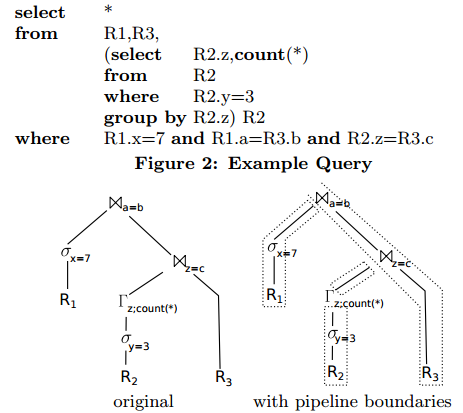
\includegraphics[width=\textwidth]{img/pipeline-boundary-1.png}
    \caption{A query with corresponding expression tree.}
    \label{fig:pipeline-boundary-1} 
  \end{subfigure}
  \begin{subfigure}{0.45\textwidth}
    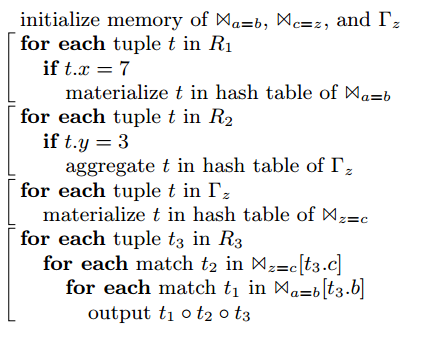
\includegraphics[width=\textwidth]{img/pipeline-boundary-2.png}
    \caption{Execution plan that avoids uneccesary materialization steps.}
    \label{fig:pipeline-boundary-2} 
  \end{subfigure}
  \caption{Neumann \ea~propose a system where queries are compiled into machine code using the LLVM compiler framework. (a) shows a sample query with corresponding expression tree. (b) shows how the query can be compiled into an execution plan that avoids unecessary materialization steps. Instead of storing intermediate results to memory for every operator in the execution tree, certain operations are performed together (data-centric execution). Courtesy of \cite{Neumann2011-uq}.} 
  \label{fig:pipeline-boundary} 
\end{figure}

Neumann \ea~have identified the need for machine code compilation of queries \cite{Neumann2011-uq}. Even though vectorized execution has come a long way to utilize modern CPUs, it is frequently outperformed by handwritten execution plans. The main reason for the performance difference is that hand-written queries are data-centric and not operator-centric, which in practice means such queries avoid unnecessary materialization steps. To counter the challenges with vectorized execution, and turn queries data-centric, Neumann \ea~propose a system where queries are compiled into machine code using the LLVM compiler framework.

As seen in Figure \ref{fig:pipeline-boundary}, the compiled queries may execute several operators from the execution tree in the same step. For instance, the filter operations are performed at in the same steps as the hash tables are built, and joining $R_1$, $R_2$, and $R_3$ is done at the same time in a nested loop. The generated execution plans are more efficient. However, the most important aspect is that the plans do not store data to memory (materialize) before it is needed. Besides, the generated code has tight loops with good code locality.

\subsection{Macro Expansions}
\label{sub:Macro Expansions}
\afigure{img/macro-expansion.png}{Macro expansions in \monetdb. For different algorithms and data types, the \texttt{select} operator has a total of 173 implementations. Courtesy of \cite{Boncz2002-yj}.}{fig:macro-expansion}{0.6}

\monetdb~uses macro expansion to reduce layers of indirection and to optimize query execution performance \cite{Boncz2002-yj}. Since operators normally are type-generic, \monetdb~has for each algorithm multiple implementations that are specific to a certain type. The implementations are generated automatically using macros, which is why they are called \textit{macro expansions}. Figure \ref{fig:macro-expansion} shows how the \texttt{select} operator is expanded into 173 implementations, depending on which algorithm and data types are queried.

The vector data structure in \ibm~is implemented using C++ templates to support multiple data types.

\section{Cache Awareness and Prefetching}
\label{sec:Cache Awareness and Prefetching}

We saw in Section \ref{sub:CPU Caches} that efficient utilization of caches is important for database performance, so data structures and algorithms should be designed such that they are cache-aware. Our research has identified several systems that are designed to be cache-aware, including \monetdb~\cite{Boncz2002-yq}, \mssql~\cite{Lahiri2015-mz}, and \ibm~\cite{Raman2013-em}. The developers of \exasol, the top performing database system in the TPC-H benchmark, claim that high level of data locality is one of the key factors to performance.

radix-cluster bla bla \todo{Input here about radix cluster algorithm if time}.

Prefetching is another way of improving cache performance. Prefetching is the technique where data is proacively loaded into the CPU caches such that it is available when an instruction needs it. Prefetching can be done automatically by a processor or a compiler, but explicit prefetching CPU instructions exist. Explicit prefetching is used by several systems studied in this research, including \ibm~\cite{Raman2013-em}, \monetx~\cite{Boncz2005-wj}, and \exasol~\cite{Exasol2014-xh}.

\section{Chapter Conclusion}
\label{sec:Chapter Conclusion}
In this chapter, we see that careful implementation is required for a high-performance, in-memory database. The implementation should utilize modern CPUs by reducing branches, function invocations, and dependencies between instructions. In addition to this, algorithms and data structures should be made \textit{cache-aware}. 

We point at \textit{vectorized execution} as the most promising technique to improve database performance in a \bd~application, as it can drastically reduce the number of cycles per tuple by operating at multiple values at a time. \textit{Vectorized execution} enables loop unrolling and memory prefetching and minimizes cache misses. We consider this technique as relatively straight-forward to implement. \textit{Vectorized execution} should be implemented using macro expansions to avoid unnecessary layers of indirection.

We see that many systems, including \bd~product \qlikview, compile queries into machine code. This technique increases the performance of expression evaluation, avoids branches, and reduces the number of function calls. Query compilation is indeed a promising technique with potentially significant performance benefits, but we believe implementing such system as non-trivial.
